\documentclass[aspectratio=169, 14pt]{beamer}
\usetheme{TalentSprint}
\usepackage{csquotes}
\usepackage{tikz}
\usepackage{tcolorbox}
\usepackage{ragged2e}
\usepackage{geometry}
\usepackage{verbatim}

\usetikzlibrary{shapes, shadows, arrows}
\tikzstyle{block} = [rectangle, draw=darkgray, fill=blue!50!lime, text width =0.9cm,rounded corners,line width = 2pt,font =\tiny]
\tikzstyle{arrow} = [thick, ->, >=stealth, color =red!70!black,line width = 2pt]
\tikzstyle{elli} = [draw, ellipse, fill=pink!30!darkgray,draw = orange, text width=3cm, minimum height = 1mm, text centered, node distance=1cm, text = white, font = \small, line width = 2pt ]
 \title[Decision Trees]{Decision Trees}

\begin{document}
{\1
\begin{frame}
%	\title[Decision Trees]{Decision Trees}
\subtitle{Decision Model}
\maketitle
\end{frame}
}

\begin{frame}{Guess the Animal Game}
\begin{itemize}
\item I have an animal in mind
\item You can ask a set of questions. 
\item You have to guess (figure out) the animal based on my answers
\begin{itemize}
\item Of course my answers will be truthful
\end{itemize}
\end{itemize}
\end{frame}

\begin{frame}{Analyze the Question!}
\begin{itemize}
\item What questions to ask?
\item Why that question? 
\item More generally,
\begin{itemize}
\item What type of questions to ask?
\item How to decide that?
\end{itemize}
\end{itemize}
\end{frame}

\begin{frame}{Analyze this Question!}
\begin{itemize}
\item How about asking \\
	\enquote{Does it have stripes?}
\item How to decide? 
\item Let us look at some data
\end{itemize}
\end{frame}


\begin{frame}{Guess the Animal -- Questions}
\begin{columns}
\column{5cm}
\begin{itemize}
\item How many legs
\item Does it fly?
\item Is it a wild animal?
\item Is it nocturnal
\item Fur/Feather?
\item Farm Animal?
\end{itemize}
\column{11cm}
	\transwipe<2-3>[direction=270]
	\begin{center}
		\only<1>{\hspace{0.2cm}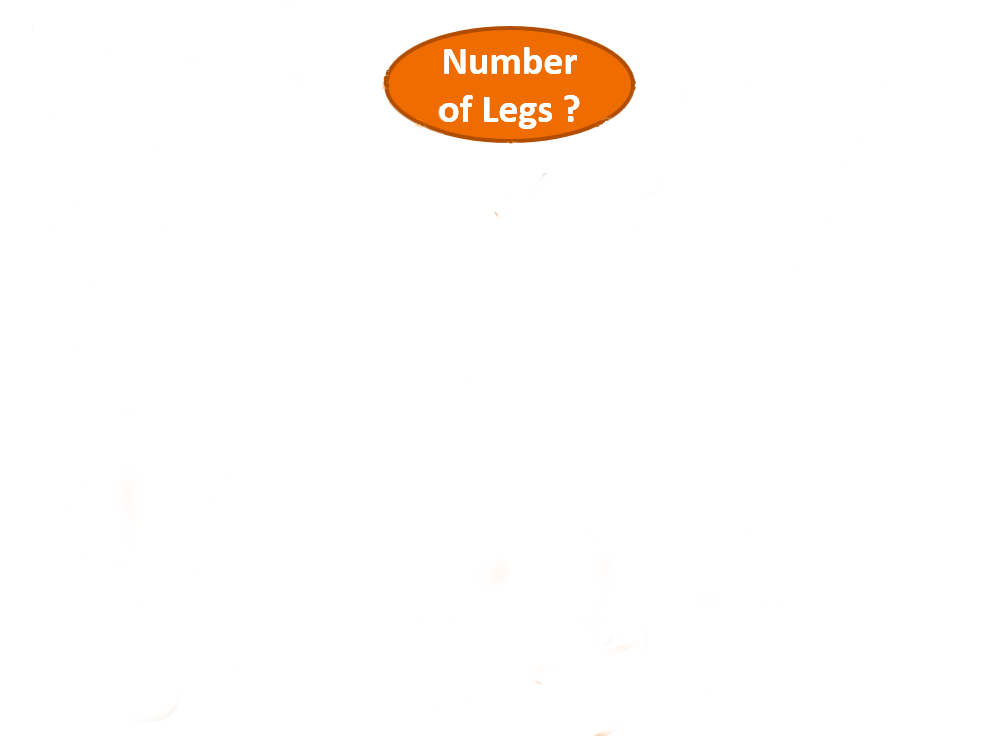
\includegraphics[width=0.7\textwidth, height=0.6\textheight]{DT_OF_Images/dtree2_5_1.png}}
	\only<2>{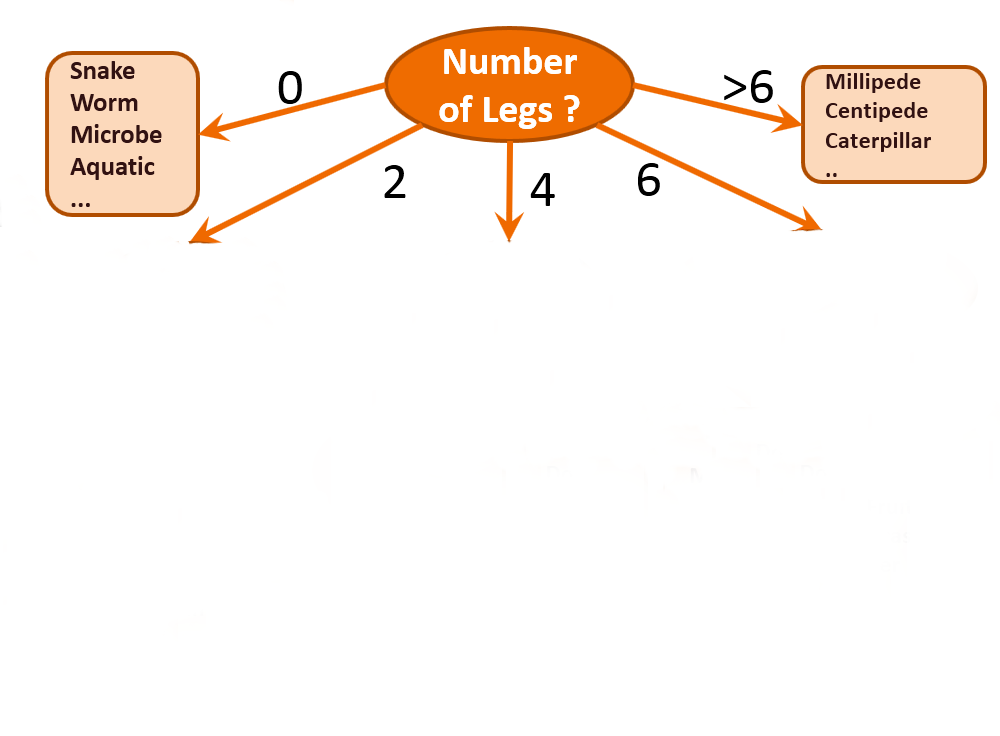
\includegraphics[width=0.7\textwidth, height=0.6\textheight]{DT_OF_Images/dtree2_5_2.png}}
	\only<3>{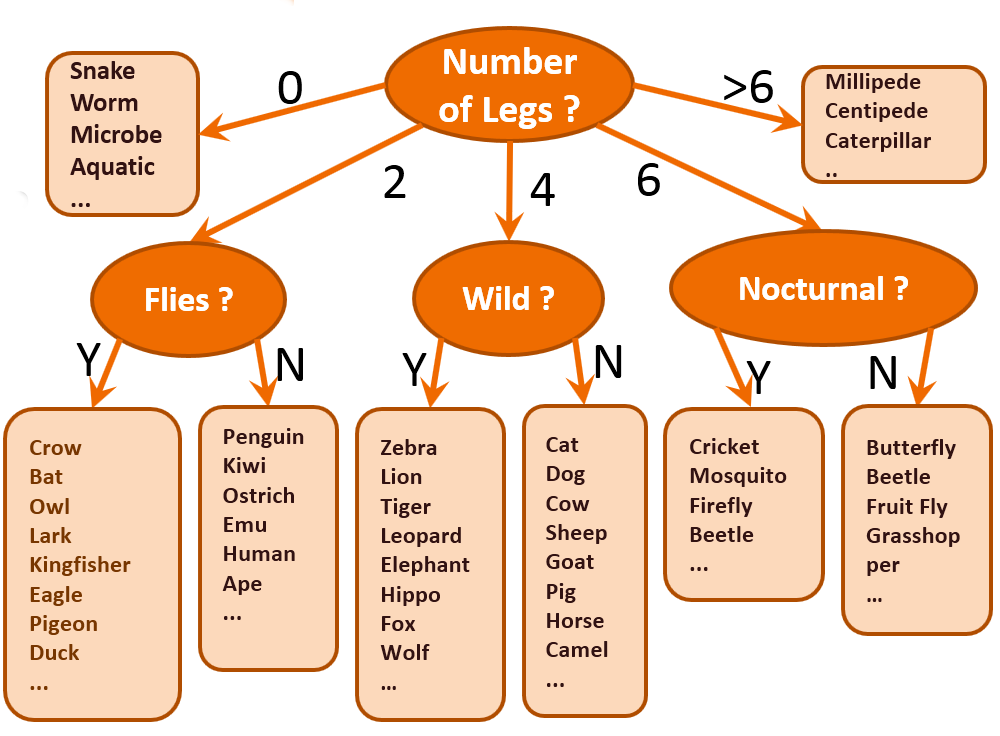
\includegraphics[width=0.7\textwidth, height=0.6\textheight]{DT_OF_Images/dtree2_5_3.png}}
	\end{center}

%        \vspace{-0.8cm}
%       \begin{center}
%\begin{tikzpicture}
%        \only<1->{\node[elli, font =\scriptsize](e1){Number of Legs?};}
%        \only<2->{\node[block, left of= e1, xshift=-5em, yshift=-0.8cm](n1){Snake Worn Microbe Aquatic...};}
%        \only<2->{\node[elli, below of = e1, yshift=-2em, text width = 1cm, xshift=-3cm, font=\scriptsize](e2){Flies?};}
%        \only<2->{\node[elli, below of = e1, yshift=-2em, text width = 1cm, xshift=0.1cm, font=\scriptsize](e3){Wild?};}
%        \only<2->{\node[elli, below of =e1, yshift=-2em,text width = 1.5cm, xshift=3cm, font=\scriptsize](e4){Noctural?};}
%        \only<2->{\node[block, right of= e1, xshift=5.5em, yshift=-0.8cm, text width = 1cm](n2){Millipede Centipede Caterpillar .....};}
%        \only<3->{\node[block, below of= e2, xshift=-1.2em, yshift=-1.5cm, text width = 0.7cm](n3){Crow Bat Owl Lark Kingfisher Eagle Pigeon Duck ..};}
%        \only<3->{       \node[block, below of= e2, xshift=1.7em, yshift=-1.2cm, text width = 0.7cm](n4){Penguin Kiwi Ostrich Emu Human Ape ....};}
%        \only<3->{       \node[block, below of= e3, xshift=-1.5em, yshift =-1.5cm, text width = 0.8cm](n5){Zebra Lion Tiger Leopard Elephant Hippo Fox Wolf..};}
%        \only<3->{      \node[block, below of= e3, xshift=1.5em, yshift =-1.5cm, text width = 0.7cm](n6){Cat Dog Cow Sheep Goat Pig Horse Camel ..};}
%        \only<3->{      \node[block, below of= e4, xshift=-1.2em, yshift =-0.9cm, text width = 1cm](n7){Cricket Mosquito Firefly Beetle ...};}
%        \only<3->{      \node[block, below of= e4,xshift=2em, yshift =-1.1cm, text width = 0.8cm](n8){Butterfly Beetle Fruit Fly Grasshopper..};}
%        \only<2->{      \draw[arrow] (e1)-- node[yshift=-0.2cm,xshift=0.7em, text=black]{0}(n1);}
%        \only<2->{      \draw[arrow] (e1)--node[yshift=-0.3cm,xshift=-0.4em, text = black]{\textgreater6}(n2);}
%        \only<2->{      \draw[arrow] (e1)--node[yshift=-0.3em, xshift=0.3em, text = black]{2}(e2);}
%        \only<2->{      \draw[arrow] (e1)--node[xshift=0.5em, text=black]{4}(e3);}
%        \only<2->{      \draw[arrow] (e1)--node[yshift=-0.3em, xshift=-0.6em, color=black]{6}(e4);}
%        \only<3->{      \draw[arrow] (e2)--node[xshift=-0.5em,yshift=0.5em, text =black]{Y}(n3);}
%        \only<3->{      \draw[arrow] (e2)--node[xshift=0.5em,yshift=0.5em,text =black]{N}(n4);}
%        \only<3->{      \draw[arrow] (e3)--node[xshift=-0.5em,yshift=0.5em, text =black]{Y}(n5);}
%        \only<3->{      \draw[arrow] (e3)--node[xshift=0.5em,yshift=0.5em,text =black]{N}(n6);}
%        \only<3->{      \draw[arrow] (e4)--node[xshift=-0.5em,yshift=0.5em, text =black]{Y}(n7);}
%        \only<3->{      \draw[arrow] (e4)--node[xshift=0.5em,yshift=0.5em,text =black]{N}(n8);}
%\end{tikzpicture}
%        \end{center}
\end{columns}

\end{frame}



\begin{frame}{Aside }
	\begin{itemize}
		\item Why Tree?
			\begin{itemize}
				\item CS Term
			\end{itemize}
		\item Related terms
			\begin{itemize}
				\item Node
				\item Sibling, child, parent
				\item Root, branch, leaf
			\end{itemize}
	\end{itemize}
\end{frame}


\begin{frame}{What is a Good Question?}
	\begin{overlayarea}{15cm}{3cm}
	\begin{itemize}
\item<2-> A question that reduces the possibilities the\, most!
\item<3-> More precisely, a question that reduces the uncertainty the most
	\end{itemize}
	
		\centering \only<4->{\alert{Mathematically, reduces the entropy the most}}
	\end{overlayarea}
\end{frame}

\begin{frame}{What is Entropy?}
	\begin{columns}
		\column{0.5\textwidth}
	\begin{itemize}
		\item<1-> Measure of \textbf{Uncertainty}
			\begin{itemize}
				\item<1-> For a set containing two classes: 
			\end{itemize}
		\transblindshorizontal<2>
				\only<2->{$$ \alert{H = -P_1\log_{2}{P_1}-P_2\log_{2}{P_2}}  $$}
			
		\item<3-> Measure of Impurity
			\begin{itemize}
				\item<3-> Not the only one
			\end{itemize}
	\end{itemize}
			\column{0.5\textwidth}
		\only<2->{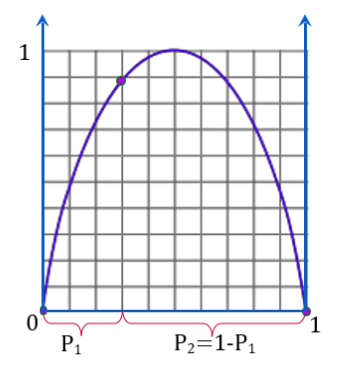
\includegraphics[width=0.9\textwidth, height=0.7\textheight]{DT_OF_Images/dtree2_8.png}}
	\end{columns}
\end{frame}



\begin{frame}[t]{Impurity Metrics}
	\begin{columns}
		\column{0.55\textwidth}
		\begin{itemize}
			\item \textbf{Entropy:}
				$ \alert{H(x)= -\sum\limits_{i = 0}^{j} P(i)\log_{2}{P(i)}}   $
			\item \textbf{GINI} 
				$\alert{ I(P) = \sum\limits_{i = 0}^{j} P_i(1-P_i)=1-\sum\limits_{i = 0}^{j}p_i^2} $
		\end{itemize}
		\column{0.45\textwidth}
		        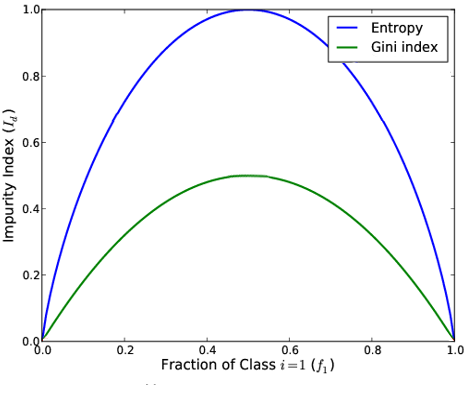
\includegraphics[width=0.9\textwidth, height=0.6\textheight]{DT_OF_Images/dtree2_9.png}
	\end{columns}
\centering	 \tiny{\textcolor{blue}{imagesource:https://www.commonlounge.com/discussion/ee8b074936a041f2b5a57d2054dc3701}}


\end{frame}


\begin{frame}[c]{Experiment}
	\begin{itemize}
		\item {Demo\_Entropy\_Animals}
			\begin{itemize}
				\item Dataset : Animals
				\item Objective : To understand how to calculate the entropy
			\end{itemize}

	\end{itemize}
\end{frame}


\begin{frame}[t]{ \hspace{2ex} Initial Entropy}


\begin{columns}
%\setlength{\columnsep}{0.1cm}		
	\column{8cm}
	\vspace{-0.5cm}
	\begin{center}
		\only<2>{
	\begin{tcolorbox}[width=0.8\textwidth,sharp corners,height=0.5\textheight,colframe=orange, colback=lime!40!blue]		
		\only<2>{\textcolor{white}{\vspace{-0.17cm}		\small{\flushleft \only<1->{Initial Entropy}}
		\begin{flushright}
			\vspace{-0.865cm}
			$= -\frac{10}{91} \log_{2}{(\frac{10}{91})}$\\
			\hfill $-\frac{10}{91} \log_{2}{(\frac{10}{91})}$\\
			\hfill $-\frac{10}{91} \log_{2}{(\frac{10}{91})}$\\
			\hfill $-\frac{10}{91} \log_{2}{(\frac{10}{91})}$\\
			\hfill $-\frac{51}{91} \log_{2}{(\frac{10}{91})}$\\
		\end{flushright}} \vspace{-20pt}
		\begin{flushright} $\small{\textbf{\textcolor{white}{= 1.86}}}$ \end{flushright} 
%			\vspace{0.8cm}\begin{flushright} $\only<1>{3.579} $ 
%		\end{flushright}
		}
	\end{tcolorbox}}
	\end{center}
	\column{7cm}
	\vspace{-0.3cm}
	\only<1->{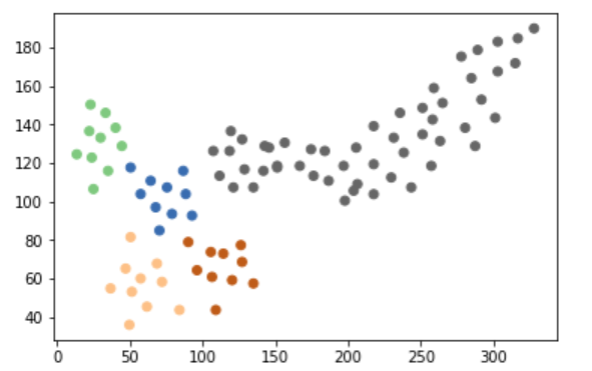
\includegraphics[width=7cm, height=0.55\textheight]{DT_OF_Images/dtree2_11.png}}
\end{columns}
\end{frame}

\begin{frame}{Which split is better?}
\end{frame}


\begin{frame}[t]{ \hspace{2ex} Which split is better?}

\centering	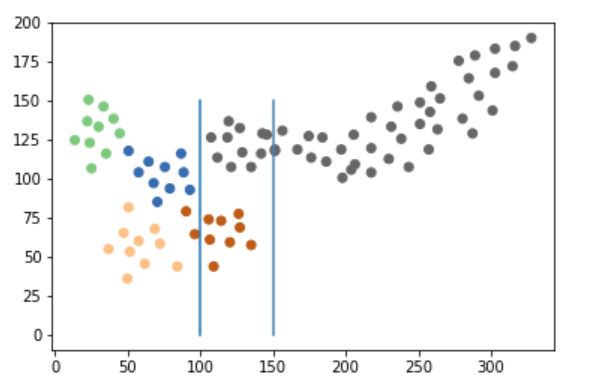
\includegraphics[width=0.7\textwidth, height=0.6\textheight]{DT_OF_Images/dtree2_12.png}

\end{frame}



\begin{frame}[t]{ \hspace{2ex} Entropy for the split -1} 
\begin{columns}	
\column{0.6\textwidth}
%	\only<1>{\centering{\begin{tcolorbox}[width=0.7\textwidth,sharp corners,height=0.07\textheight,colframe=orange, colback=lime!60!blue]
%		\centering	\tiny{\textbf{Initial Entropy 3.579}}
%	\end{tcolorbox}}}
%	\only<1>{\begin{tcolorbox}[width=8.4cm,sharp corners,height=0.155\textheight,colframe=orange, colback=lime!60!blue]
%	\vspace{0.5cm} \centering \tiny{\textbf{(Left side Entropy)}}
%	\end{tcolorbox}}
%	\only<1>{\begin{tcolorbox}[width=0.7\textwidth,sharp corners,height=0.15\textheight,colframe=orange, colback=lime!60!blue]
%        \vspace{0.5cm} \centering \tiny{\textbf{(Right side Entropy)}}
%	\end{tcolorbox}}
%	\only<1>{\begin{tcolorbox}[width=0.7\textwidth,sharp corners,height=0.07\textheight,colframe=orange, colback=lime!60!blue]
%		\centering     \tiny{\textbf{Total Entropy =+ = 2.322}}
%	\end{tcolorbox}}
	\only<1>{\vspace{-4.3cm}}
	\only<1->{\centering{\begin{tcolorbox}[width=0.7\textwidth,sharp corners,height=0.07\textheight,colframe=orange, colback=lime!70!blue]
    \centering      \tiny{\textbf{Initial Entropy=1.86}}
     \end{tcolorbox}}}
	\only<2->{\begin{tcolorbox}[width=7.3cm, sharp corners,height=0.19\textheight,colframe=orange, colback=lime!70!blue]
		\tiny{\textbf{$H_1 = -\frac{10}{51}\log_{2}{(\frac{10}{51})}-\frac{10}{51}\log_{2}{(\frac{10}{51})}-\frac{10}{51}\log_{2}{(\frac{10}{51})}-\frac{10}{51}\log_{2}{(\frac{10}{51})}-\frac{11}{51}\log_{2}{(\frac{11}{51})}$}} \vspace{-0.15cm} \centering	$$\textbf{\tiny{=2.322(Left side Entropy)}}$$
	\end{tcolorbox}}
	\only<2->{\begin{tcolorbox}[width=0.7\textwidth,sharp corners,height=0.15\textheight,colframe=orange, colback=lime!70!blue]
		\tiny{\textbf{$H_2 = -\frac{40}{40}\log_{2}{(\frac{40}{40})}=-1\log_{2}{1}$} \vspace{-5pt} \centering \tiny{$$\textbf{=0(Right side Entropy)}$$}}
	\end{tcolorbox}}
	\only<2->{\begin{tcolorbox}[width=0.7\textwidth,sharp corners,height=0.1\textheight,colframe=orange, colback=lime!70!blue]
		\centering      \tiny{\textbf{Total Entropy = $(\frac{51}{91})H_1+(\frac{40}{91})H_2 = 1.301 $}}
	\end{tcolorbox}}

\column{0.4\textwidth}

	\only<1->{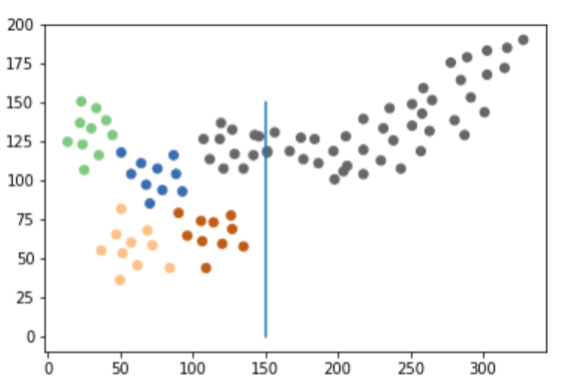
\includegraphics[width=\textwidth, height=0.6\textheight]{DT_OF_Images/dtree2_13.png}}
	\only<2>{\vspace{-0.01cm}}
\end{columns}


\end{frame}

\begin{frame}[t]{ \hspace{2ex} Entropy for the split -2}
\begin{columns}
\column{0.6\textwidth}

	\only<1->{\centering{\begin{tcolorbox}[width=0.7\textwidth,sharp corners,height=0.07\textheight,colframe=orange, colback=lime!70!blue]
		\centering      \tiny{\textbf{Initial Entropy=1.86}} 
	\end{tcolorbox}}}
 \only<1>{\vspace{3cm}}


	\only<2->{\begin{tcolorbox}[width=7.5cm,sharp corners,height=0.2\textheight,colframe=orange, colback=lime!70!blue]
\centering	     \tiny{\textbf{$H_1 = -\frac{10}{32}\log_{2}{(\frac{10}{32})}-\frac{10}{32}\log_{2}{(\frac{10}{32})}-\frac{10}{32}\log_{2}{(\frac{10}{32})}-\frac{2}{32}\log_{2}{(\frac{2}{32})}$}} \vspace{-5pt} \centering    $$\textbf{\tiny{=1.823(Left side Entropy)}}$$
        \end{tcolorbox}}
	\only<2->{\begin{tcolorbox}[width=0.7\textwidth,sharp corners,height=0.15\textheight,colframe=orange, colback=lime!70!blue]
		\tiny{\textbf{$H_2 = -\frac{8}{59}\log_{2}{(\frac{8}{59})}-\frac{51}{59}\log_{2}{(\frac{51}{59})}$}} \vspace{-10pt} \centering \tiny{$$\textbf{=0.571(Right side Entropy)}$$}
        \end{tcolorbox}}
        \only<2->{\begin{tcolorbox}[width=0.7\textwidth,sharp corners,height=0.1\textheight,colframe=orange, colback=lime!70!blue]
		\centering      \tiny{\textbf{Total Entropy = $ (\frac{32}{91})H_1+(\frac{59}{91})H_2 = 1.011 $}}
        \end{tcolorbox}}


\column{0.4\textwidth}

\only<1->{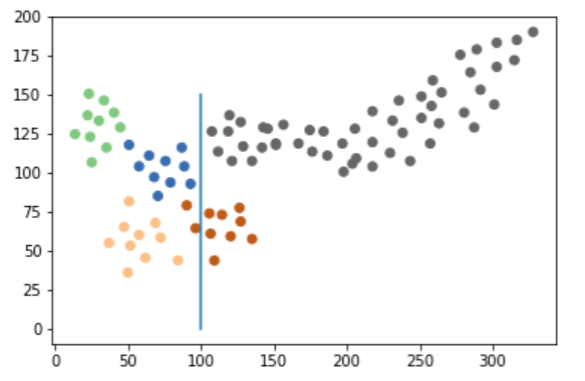
\includegraphics[width=6.36cm, height=0.6\textheight]{DT_OF_Images/dtree2_14.png}}
	\only<1>{\vspace{-2cm}}
	\only<2>{\vspace{-0.45cm}}
	\column{0.03\textwidth}

\end{columns}

\end{frame}

\begin{frame}[t,fragile]{\hspace{3ex}DT in Scikit Learn}
\alert{Training:}
\begin{verbatim}
from sklearn.tree import DecisionTreeClassifier
clf = DecisionTreeClassifier(criterion = "entropy",
        	max_depth = 5)
				clf.fit(x_train, y_train)
				Z = clf.predict(x,y)
		\end{verbatim}

%\begin{tikzpicture}[remember picture,overlay]
%\node[anchor=south east,xshift=1pt,yshift=4.5pt] at (current page.south east) {\href{https://drive.google.com/file/d/1N2M-5G0DFp9VRCwdELygiPuP2K2Z7ND5/view}{
\includegraphics[height=1cm]{bottom.png}}};
%\end{tikzpicture}
\end{frame}

\begin{frame}{(Dis)advantages of Decision Trees }
	\begin{columns}
		\column{7cm}
		\begin{itemize}	
				\small
			\item Fast, Compact and Effective
			\item Handles categorical variables *
			\item Interpretable as a set of rules
			\item Can indicate the most useful features
			\end{itemize}
		\hspace{1cm}		\small{\alert{*Sklearn doesn\rq t support}}
			\column{9cm}
			\begin{itemize}
					\vspace{-1cm}	\small
			\item Not suitable for prediction of continuous attribute 
			\item Does not handle non-rectangular regions well
			\item Computationally expensive to train
			\item Tends to overfit
			\end{itemize}
	\end{columns}
\end{frame}


\begin{frame}{Experiment}
	\begin{itemize}
	    \item {Demo\_DT\_Overfitting}
			\begin{itemize}
				\item Objective : To understand how a decision tree classifier can overfit the data
			\end{itemize}
	
	\end{itemize}
\end{frame}


\begin{frame}{DT\_Overfitting}
	\begin{columns}
		\column{5cm}
		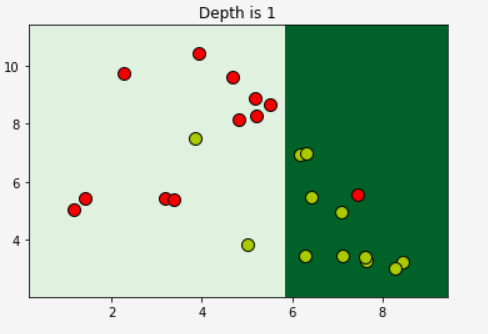
\includegraphics[width=\textwidth, height=0.6\textheight]{DT_OF_Images/dtree2_22.png}
		\column{5cm}
		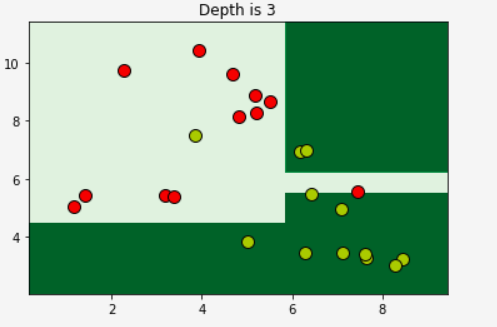
\includegraphics[width=\textwidth, height=0.6\textheight]{DT_OF_Images/dtree2_22a.png}
		\column{5cm}
		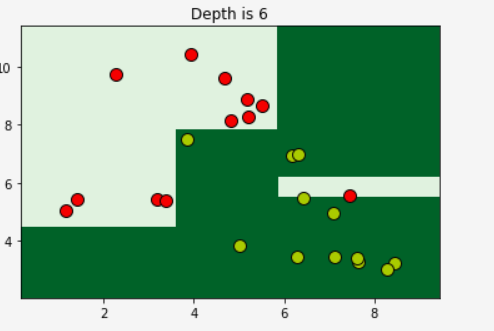
\includegraphics[width=\textwidth, height=0.6\textheight]{DT_OF_Images/dtree2_22b.png}

	\end{columns}
\end{frame}

\begin{frame}{Overfitting Example}
\centering
	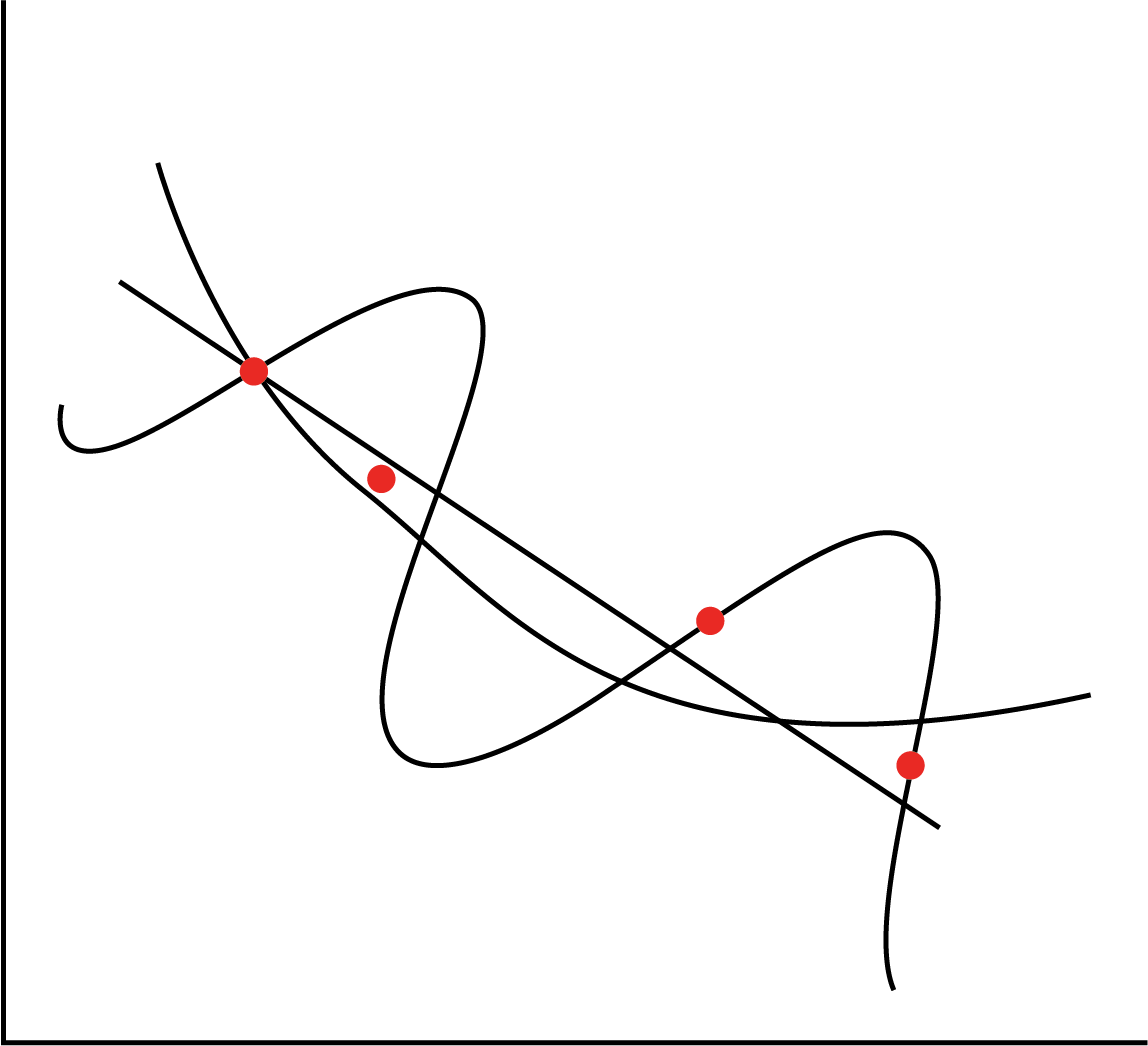
\includegraphics[width=0.5\textwidth, height=0.7\textheight]{DT_OF_Images/dtree2_23.png}

\end{frame}


\begin{frame}[t]{Early Stopping and Pruning}
	\vspace{-0.2cm}	\begin{itemize}
		\item Decision trees are notorious for overfitting
		\item Early Stopping
			\begin{itemize}
				\item Do not split beyond a point
			\end{itemize}
		\item Pruning
			\begin{itemize}
				\item Once the tree is formed, remove weakest branches
				\item Use validation set to decide when to stop
			\end{itemize}
				\item Both approaches also reduce the depth and improve  classification speed
	\end{itemize}

\end{frame}


\begin{frame}{Decision Tree Classifier Parameters}
	\begin{itemize}
		\item Early Stopping \textbf{- min\_impurity\_split}
			\begin{itemize}
				\item Threshold for early stopping in tree growth
			\end{itemize}
		\item Prunning \textbf{- min\_samples\_leaf}
			\begin{itemize}
				\item The minimum number of samples required to be at leaf node
				\item This parameter helps limit the growth of the tree
			\end{itemize}
	\end{itemize}
\end{frame}


\begin{frame}{Handling missing values}
	\begin{itemize}
		\item Impute values
			\begin{itemize}
				\item Impute 0
				\item Mean/median imputation
				\item Impute from observed values: build predictor
				\item Impute from last observation
	\end{itemize}
	\end{itemize}
	\end{frame}
\begin{frame}[t]{Applications of Decision Trees}
	\begin{itemize}
		\item Medical diagnosis
		\item Credit risk analysis
	\end{itemize}
\end{frame}
{\1
\begin{frame}
	\title{Thanks!!}
	\subtitle{Questions?}
	\titlepage
\end{frame}

}

\end{document}
